\section{Problems}

\subsection{Statement of the Problems}

Many citizens find themselves under the pressure over moderate and too busy to pursue for happiness. They are in unhealthy mental conditions but lack for convenient ways to get happiness. People have tried to get happiness since the happiness lesson in Haward, aiming to teach people to be happy, has become one of the most popular courses. According to China Daily, many high school students find themselves under high pressure, which is shown in the graph below. Even though they want to do some exercise sometimes, the space is limited.
\begin{figure}
    \centering
    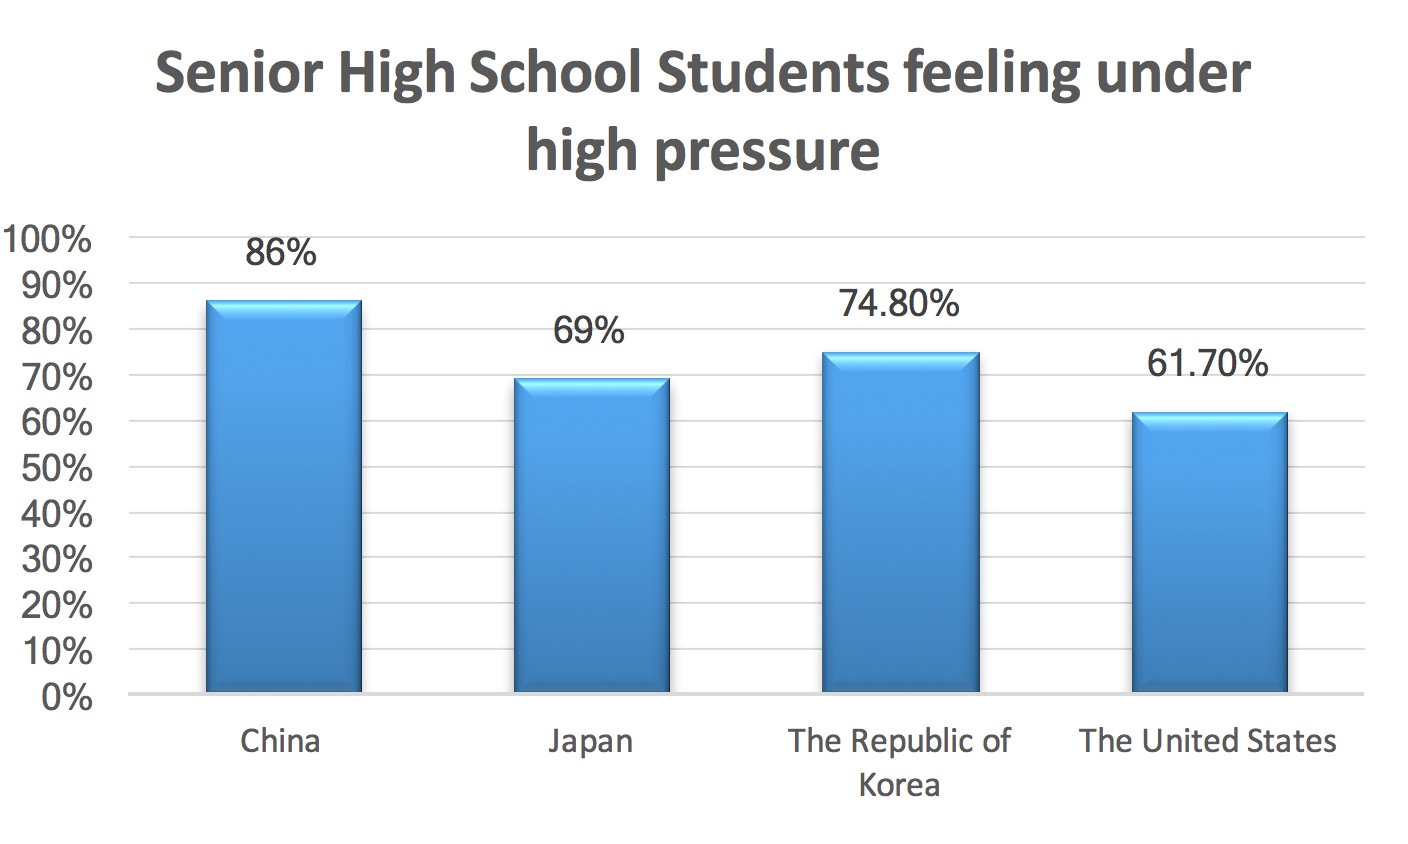
\includegraphics[width=13cm]{Pics/Problems1}
    \caption{Proportion of Senior High School Students under High Pressure}
    \label{scalerStep}
\end{figure}

